% !TEX root =  ../main_manuscript.tex 
\section{Application of Personalized Schedules in Prostate Cancer Surveillance}
\label{sec:results}
We next demonstrate personalized schedules for scheduling biopsies in prostate cancer active surveillance. To this end, we reuse results from a joint model we previously fitted~\citep{tomer2019personalized} to the PRIAS dataset introduced in Section~\ref{subsec:motivational_study}. This model utilized a linear mixed sub-model for biannually measured PSA (continuous: log-transformed from ng/mL), and a logistic mixed sub-model for biannually measured DRE (binary: tumor palpable or not). The model employed B-splines~\citep{de1978practical} to accommodate non-linear PSA evolution over follow-up. In the survival sub-model, fitted PSA value, fitted instantaneous PSA velocity (defined in Section~\ref{subsec:surival_sub_model}), and log-odds of having a DRE indicating a palpable tumor, were included as time-dependent predictors. The model parameters were estimated under the Bayesian framework~\citep{tomer2019personalized} using the R package \textbf{JMbayes}~\citep{rizopoulosJMbayes}. While the full model definition, and parameter estimates are provided in~\citet{tomer2019personalized}, we next briefly present the key results relevant for personalized scheduling.

First, the cumulative-risk of progression at the maximum study period of ten years was 50\% (Web-Figure~1). This indicates that many patients may not require all the annual biopsies they are currently prescribed. Since personalized schedules are risk-based, their overall performance is dependent on the predictive accuracy and discrimination capacity of the fitted model. In this regard, the model had a moderate area under the receiver operating characteristic curve (AUC) over the follow-up period (between 0.61 and 0.68). The mean absolute prediction error was moderate to large (between 0.08 and 0.24) and decreased rapidly after year one of follow-up. Thus, personalized schedules based on this model may work better after year one with more follow-up data.

\subsection{Personalized Biopsy Schedules for a Demonstration Prostate Cancer Patient}
We utilized the joint model fitted to the PRIAS dataset to schedule biopsies in a demonstration PRIAS patient (Figure~\ref{fig:demo_schedule}), starting from his current visit at year five, until year ten of follow-up. This patient has not progressed until year 3.5, and hence even if he incurs a delay in detecting progression of up to three years, it may not lead to adverse outcomes~\citep{carvalho}. Also, since his cumulative-risk of progression at year ten is only 18.8\%, he is likely to progress slowly. Consequently, risk-based fewer biopsies are planned in risk-based personalized schedules than the widely used annual schedule (Panel~B, Figure~\ref{fig:demo_schedule}). In addition, in both personalized schedule based on a fixed risk threshold of 10\% and automatically chosen risk threshold $\kappa^*(v)$, the expected delay in detecting progression is much less the aforementioned limit of three years (Panel~D, Figure~\ref{fig:demo_schedule}).

The current PRIAS protocol for biopsies is fixed biopsies at year one, four, seven, and ten of follow-up, and every five years after that. Additional annual biopsies are scheduled if a patient's PSA doubling-time~\citep{bokhorst2015compliance} is high.
Our event of interest is cancer progression.

\begin{figure}
\centerline{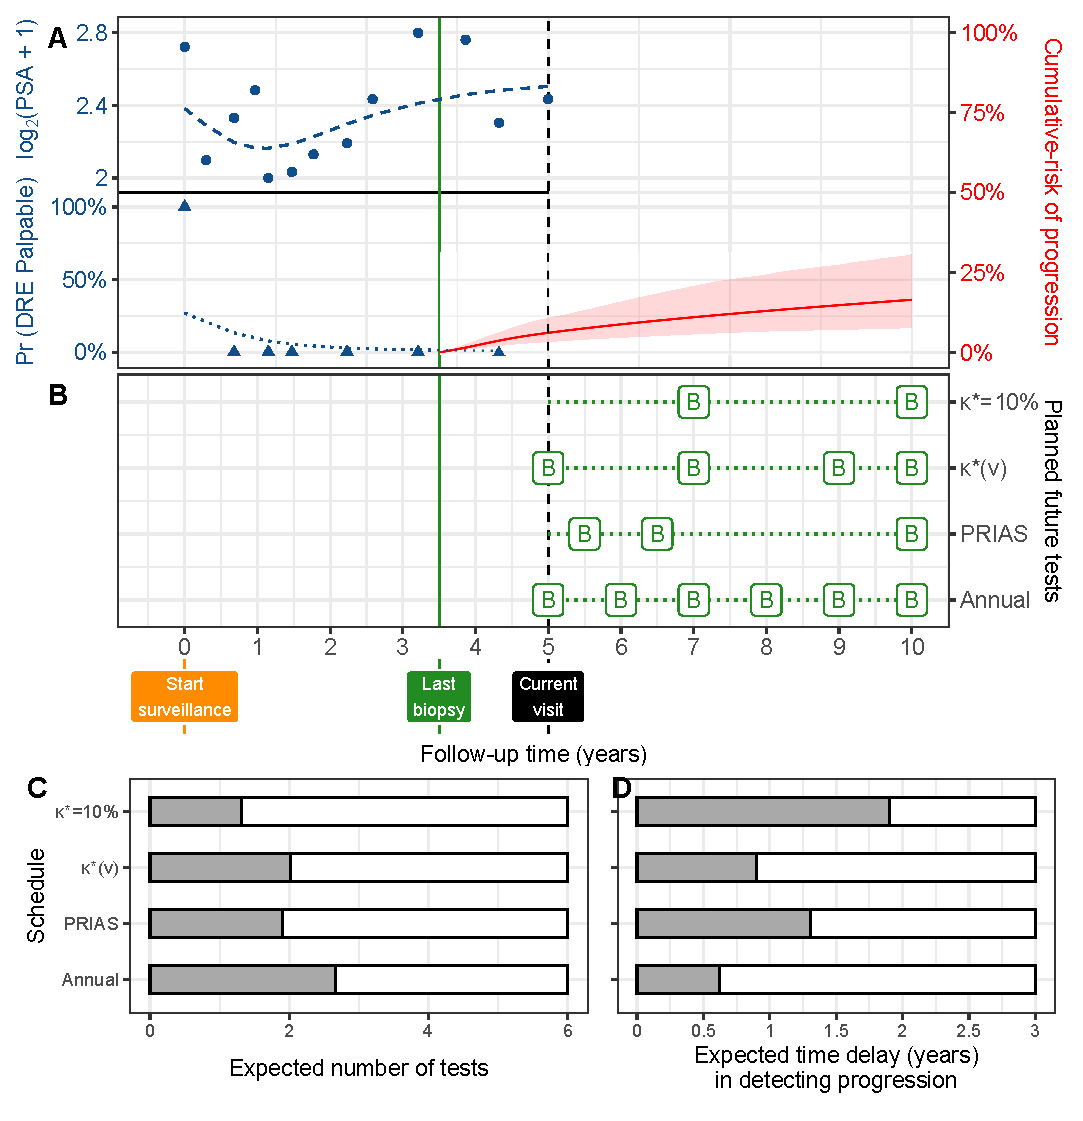
\includegraphics{images/demo_schedule.eps}}
\caption{\textbf{Illustration of personalized schedules for a demonstration PRIAS patient:} In \textbf{Panel~A}: Time of last negative biopsy is year 3.5 (vertical green solid line). Longitudinal data: DRE (blue triangles) and PSA (blue circles). The current visit is year five (vertical black dashed line). The estimated cumulative-risk profile is shown with a solid red line (95\% credible interval is shaded). It is 18.8\% at year ten (horizon). In \textbf{Panel~B}, we visualize different biopsy schedules, with a `B' indicating a biopsy. \textbf{$\kappa=10\%$} and \textbf{$\kappa^*(v)$} are personalized biopsy schedules using a fixed risk threshold of 10\%, and automatically chosen threshold~(\ref{eq:kappa_choice}), respectively. PRIAS and Annual denote the PRIAS biopsy schedule (paragraph~2 of Section~\ref{sec:results}) and annual biopsy schedule. \textbf{Panel~C,D}: For all schedules we calculate the expected number of tests and expected time delay in detecting progression if the patient progresses before year ten. Since a recommended minimum gap of one year is maintained between biopsies, maximum possible number of tests are six.  A delay in detecting progression of up to three years may not lead to adverse outcomes~\citep{carvalho}. }\label{fig:demo_schedule}
\end{figure}